\documentclass[compress]{beamer}
\usepackage{ifthen,verbatim}

\newcommand{\isnote}{}
\xdefinecolor{lightyellow}{rgb}{1.,1.,0.25}
\xdefinecolor{darkblue}{rgb}{0.1,0.1,0.7}

%% Uncomment this to get annotations
%% \def\notes{\addtocounter{page}{-1}
%%            \renewcommand{\isnote}{*}
%% 	   \beamertemplateshadingbackground{lightyellow}{white}
%%            \begin{frame}
%%            \frametitle{Notes for the previous page (page \insertpagenumber)}
%%            \itemize}
%% \def\endnotes{\enditemize
%% 	      \end{frame}
%%               \beamertemplateshadingbackground{white}{white}
%%               \renewcommand{\isnote}{}}

%% Uncomment this to not get annotations
\def\notes{\comment}
\def\endnotes{\endcomment}

\setbeamertemplate{navigation symbols}{}
\setbeamertemplate{headline}{\mbox{ } \hfill
\begin{minipage}{5.5 cm}
\vspace{-0.75 cm} \small
\end{minipage} \hfill
\begin{minipage}{4.5 cm}
\vspace{-0.75 cm} \small
\begin{flushright}
\ifthenelse{\equal{\insertpagenumber}{1}}{}{Jim Pivarski \hspace{0.2 cm} \insertpagenumber\isnote/\pageref{numpages}}
\end{flushright}
\end{minipage}\mbox{\hspace{0.2 cm}}\includegraphics[height=1 cm]{../cmslogo} \hspace{0.1 cm} \includegraphics[height=1 cm]{../tamulogo} \hspace{0.01 cm} \vspace{-1.05 cm}}

\begin{document}
\begin{frame}
\vfill
\begin{center}
\textcolor{darkblue}{\Large Muon Geometry for CRAFT:}

\vspace{0.2 cm}
\textcolor{darkblue}{\Large HIP Group's Perspective}

\vfill
\begin{columns}
\column{0.3\linewidth}
\begin{center}
\large
\textcolor{darkblue}{Jim Pivarski}

\vspace{0.2 cm}
Alexei Safonov
\end{center}
\end{columns}

\begin{columns}
\column{0.3\linewidth}
\begin{center}
\scriptsize
{\it Texas A\&M University}
\end{center}
\end{columns}

\vfill
19 November, 2008

\end{center}
\end{frame}

%% \begin{notes}
%% \item This is the annotated version of my talk.
%% \item If you want the version that I am presenting, download the one
%% labeled ``slides'' on Indico (or just ignore these yellow pages).
%% \item The annotated version is provided for extra detail and a written
%% record of comments that I intend to make orally.
%% \item Yellow notes refer to the content on the {\it previous} page.
%% \item All other slides are identical for the two versions.
%% \end{notes}

\small

\begin{frame}
\frametitle{Status of muon alignment}
\begin{itemize}
\item HIP group produced a track-based alignment procedure of barrel
  wheels and endcap disks and a first set of constants in time for
  CRAFT reprocessing (November 9)
\begin{itemize}
\item including sanity checks of internal issues, like residuals $\to$
  0, run-by-run stability, etc.
\item rough agreement with MillePede's wheel measurements
\end{itemize}

\item Of course, that's not enough: we must be sure that the constants
  accord with reality

\item Muon hardware alignment system provides a powerful cross-check

\item We were told that our results were inconsistent with established
  hardware measurements/constraints
\begin{itemize}
\item If so, it {\it could} point to $\chi^2$-invariant global
  deformations of the tracker, in which case the role of track-based
  alignment could be reversed to constrain tracker

\item {\it But} we have recieved very little and very late input as to
  what the exact values of those established results are
\end{itemize}

\item As a group (track-based and hardware alignments), we'll need to
  improve our internal communication and decision-making

\end{itemize}
\end{frame}

\begin{frame}
\frametitle{Status of constants (1)}
\begin{itemize}
\item CRAFT\_V3P::All (old constants) contains
\begin{itemize}\setlength{\itemsep}{0.1 cm}
\item alignment of DT chambers within wheels from pre-CRAFT tracks and survey
\item no wheel-to-wheel or disk-to-disk corrections (large error)
\item no endcap disk-bulging
\end{itemize}

\item Track-based alignment of wheel and disk positions is cast into
  doubt because of possible global deformations of the tracker, so we
  will not provide updates

\item Laser alignment of endcap disk-bulging was well-studied, but not in a usable format
\begin{itemize}\setlength{\itemsep}{0.1 cm}
\item I converted ME$\pm$2, 3, 4 from Excel to \mbox{CSCAlignmentRcd by hand\hspace{-1 cm}}
\item Couldn't find ME$\pm$1, so I {\it guessed} approximate values
\item Formatting should be done by hardware alignment group!
\end{itemize}

\textcolor{darkblue}{\tiny \tt /afs/cern.ch/cms/CAF/CMSALCA/ALCA\_MUONALIGN/SWAlignment/CRAFTwheeldisk/CurvedEndcapsOnly.db}

\textcolor{darkblue}{\tiny \tt /afs/cern.ch/cms/CAF/CMSALCA/ALCA\_MUONALIGN/SWAlignment/CRAFTwheeldisk/CurvedEndcapsOnly.xml}

\end{itemize}
\end{frame}

\begin{frame}
\frametitle{Status of constants (2)}

\begin{itemize}\setlength{\itemsep}{0.2 cm}
\item We should also set the relative position of the tracker and
  muon system with tracks
\begin{itemize}\setlength{\itemsep}{0.1 cm}
\item tracker position is not defined in terms of a physical landmark
\item relative alignment is {\it defined} by globalMuon consistency
\item translating entire muon system cannot affect standAloneMuons
\end{itemize}

\item $-$3.8~mm correction in Tracker entry of GlobalPositionRcd:

\textcolor{darkblue}{\tiny \tt /afs/cern.ch/cms/CAF/CMSALCA/ALCA\_MUONALIGN/SWAlignment/CRAFTwheeldisk/CRAFT\_GlobalPositionRcd.db}

\item From track-based alignment of wheel~0 with full CRAFT dataset (details on next page)

\item Doesn't affect any new DT updates and doesn't change the coordinates of anything in the muon system
\end{itemize}

%% \vfill
%% \hspace{-0.83 cm} \textcolor{darkblue}{\Large Summary}

%% \vspace{0.1 cm}
%% \begin{itemize}
%% \item Can't fix wheel/disk $z$ positions (DT updates from \mbox{MillePede group?)\hspace{-1 cm}}
%% \item Can add disk-bulging (reminder: ME$\pm$1 shape was guessed!)
%% \item Can fix global $z$ position (independent of DT updates)
%% \end{itemize}
\end{frame}

\begin{frame}
\frametitle{Details of global $z$ measurement}
\begin{itemize}
\item Every globalMuon track measures tracker-muon displacement, but
  low-momentum tracks are dominated by multiple scattering (tails)
\begin{itemize}
\item want to take a mean of the highest-momentum tracks
\item plot alignment correction versus curvature ($q/p_T$)
\item Taylor-expand around infinite momentum ($q/p_T = 0$)
\item Quadratic fit: $p_0$ is misalignment (constant), $p_1$ is $\vec{B}$ error (antisymmetric with $q$), $p_2$ is multiple \mbox{scattering (symmetric with $q$)\hspace{-1 cm}}
\end{itemize}

\item Wheel~0 measurement is most reliable above $\sim$40~GeV \mbox{($|q/p_T| < 0.025$)\hspace{-1 cm}}
\end{itemize}

\vfill
\begin{columns}
\column{0.3\linewidth}
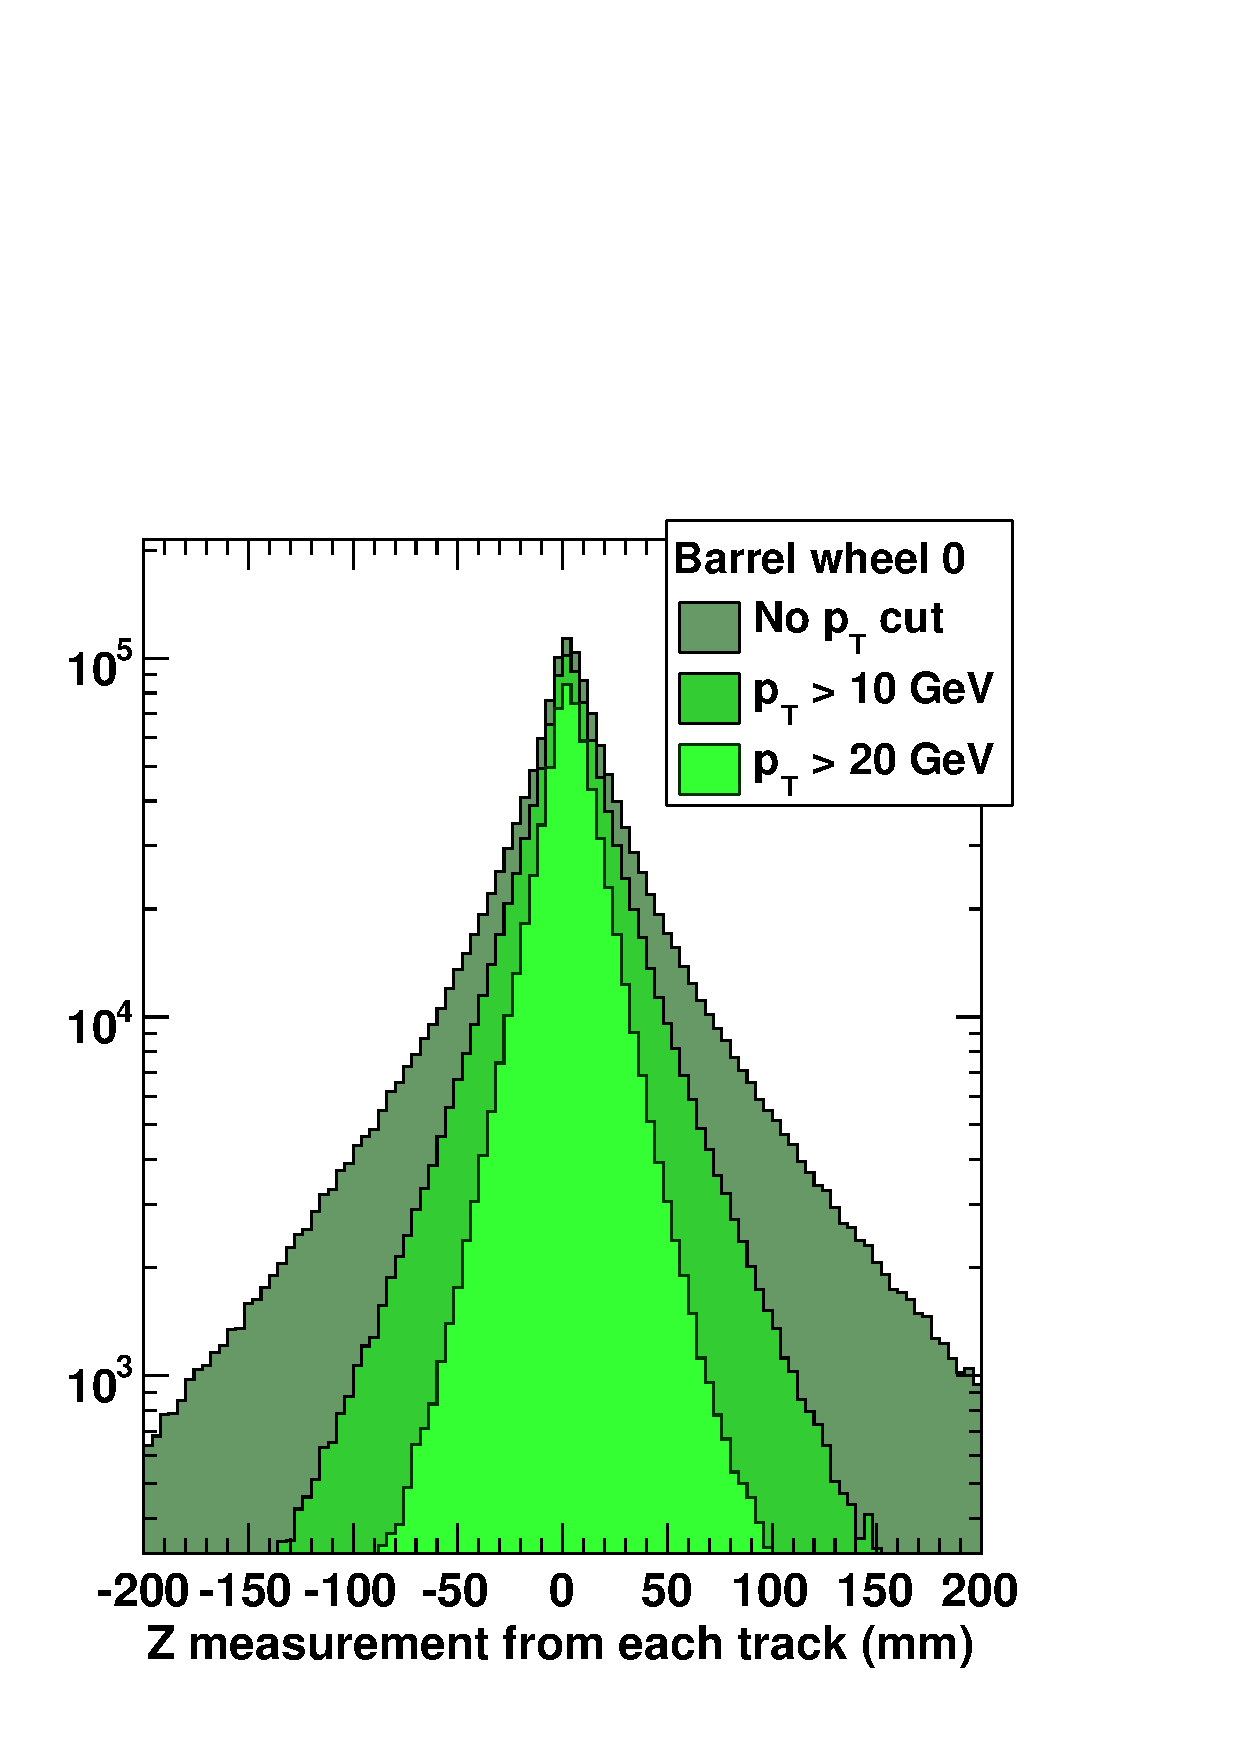
\includegraphics[width=\linewidth]{Zparameter_wh0.pdf}
\column{0.35\linewidth}
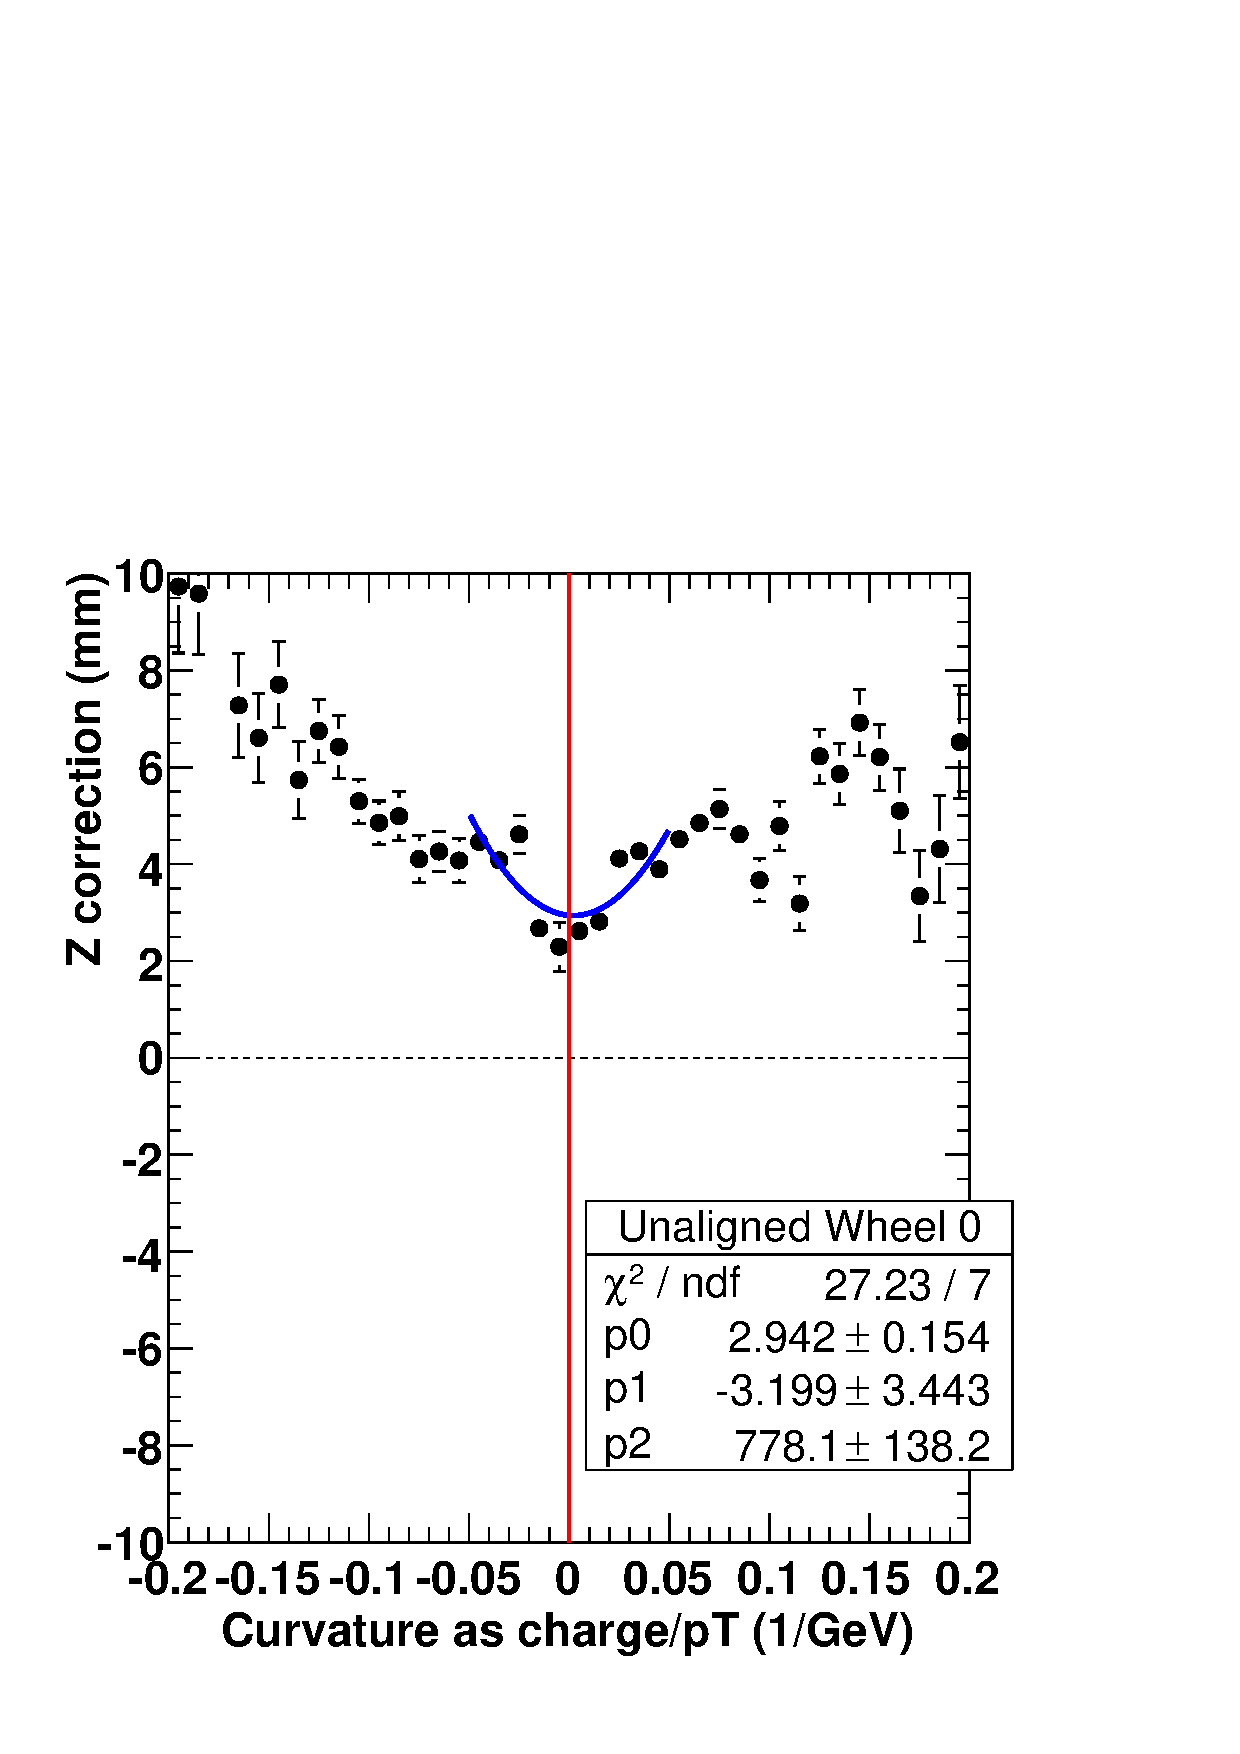
\includegraphics[width=\linewidth]{ZvsCurvature_wh0_unaligned.pdf}
\column{0.35\linewidth}
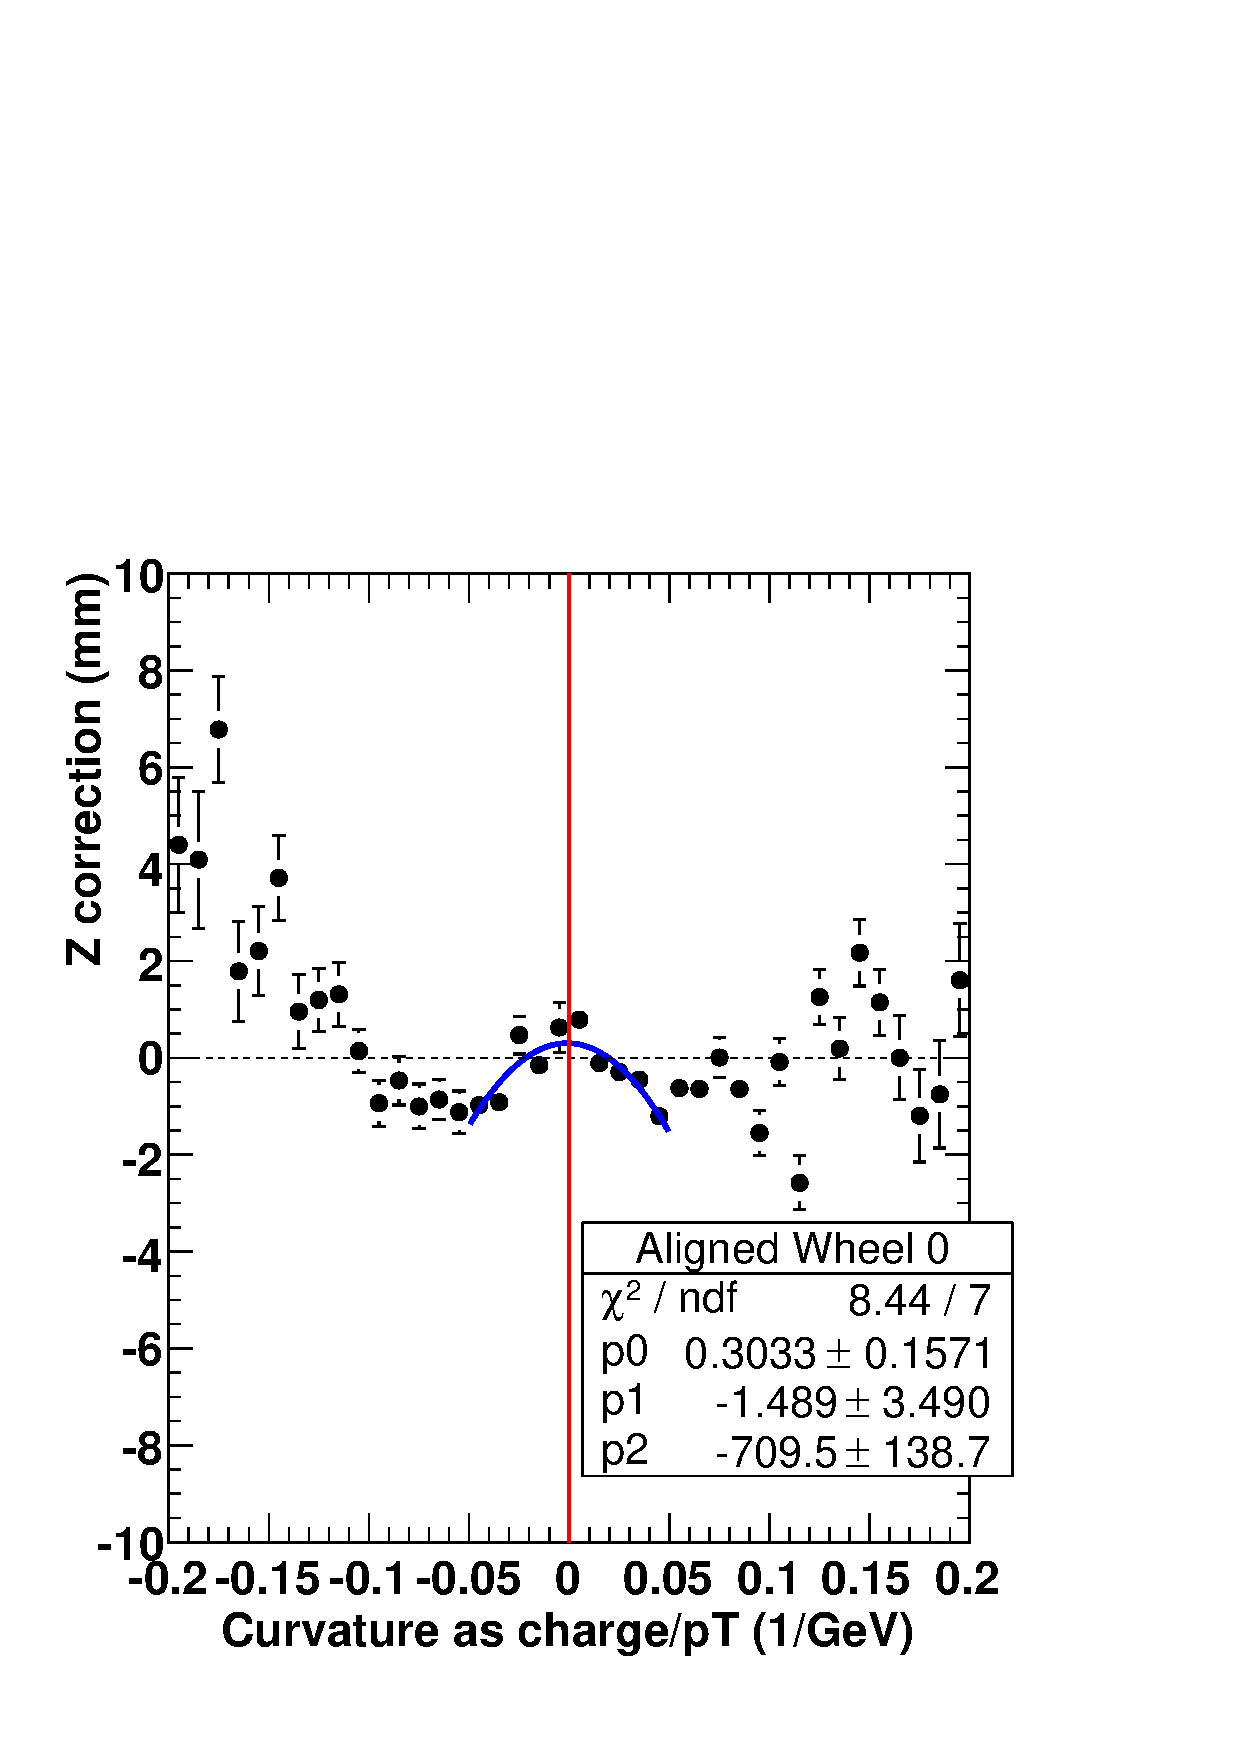
\includegraphics[width=\linewidth]{ZvsCurvature_wh0_aligned.pdf}
\end{columns}
\end{frame}

\begin{frame}
\frametitle{Conclusions}
\begin{itemize}\setlength{\itemsep}{0.25 cm}
\item Recommended endcap and global position corrections \\ (tags are named ``CSCAlignmentRcd'' and ``GlobalPositionRcd''):

\textcolor{darkblue}{\tiny \tt /afs/cern.ch/cms/CAF/CMSALCA/ALCA\_MUONALIGN/SWAlignment/CRAFTwheeldisk/CurvedEndcapsOnly.db}

\textcolor{darkblue}{\tiny \tt /afs/cern.ch/cms/CAF/CMSALCA/ALCA\_MUONALIGN/SWAlignment/CRAFTwheeldisk/CRAFT\_GlobalPositionRcd.db}

\begin{itemize}
\item Relative disk positions remain uncorrected
\end{itemize}

\item I am unfamiliar with new constants proposed for the barrel

\item While the muon alignment group as a whole needs to communicate
  better and have a more formal decision-making process, we'd like to
  emphasize that our HIP group's objective is just \mbox{track-based alignment\hspace{-2 cm}}
\begin{itemize}\setlength{\itemsep}{0.1 cm}
\item I should not be spending time trying to interpret and translate hardware results
\item About a year ago, we all agreed that hardware alignment would be
  provided as alignment records, to be a starting point for track-based alignment
\item We need to get back to that model
\end{itemize}
\end{itemize}
\label{numpages}
\end{frame}

%% \begin{columns}
%% \column{0.5\linewidth}
%% \hfill 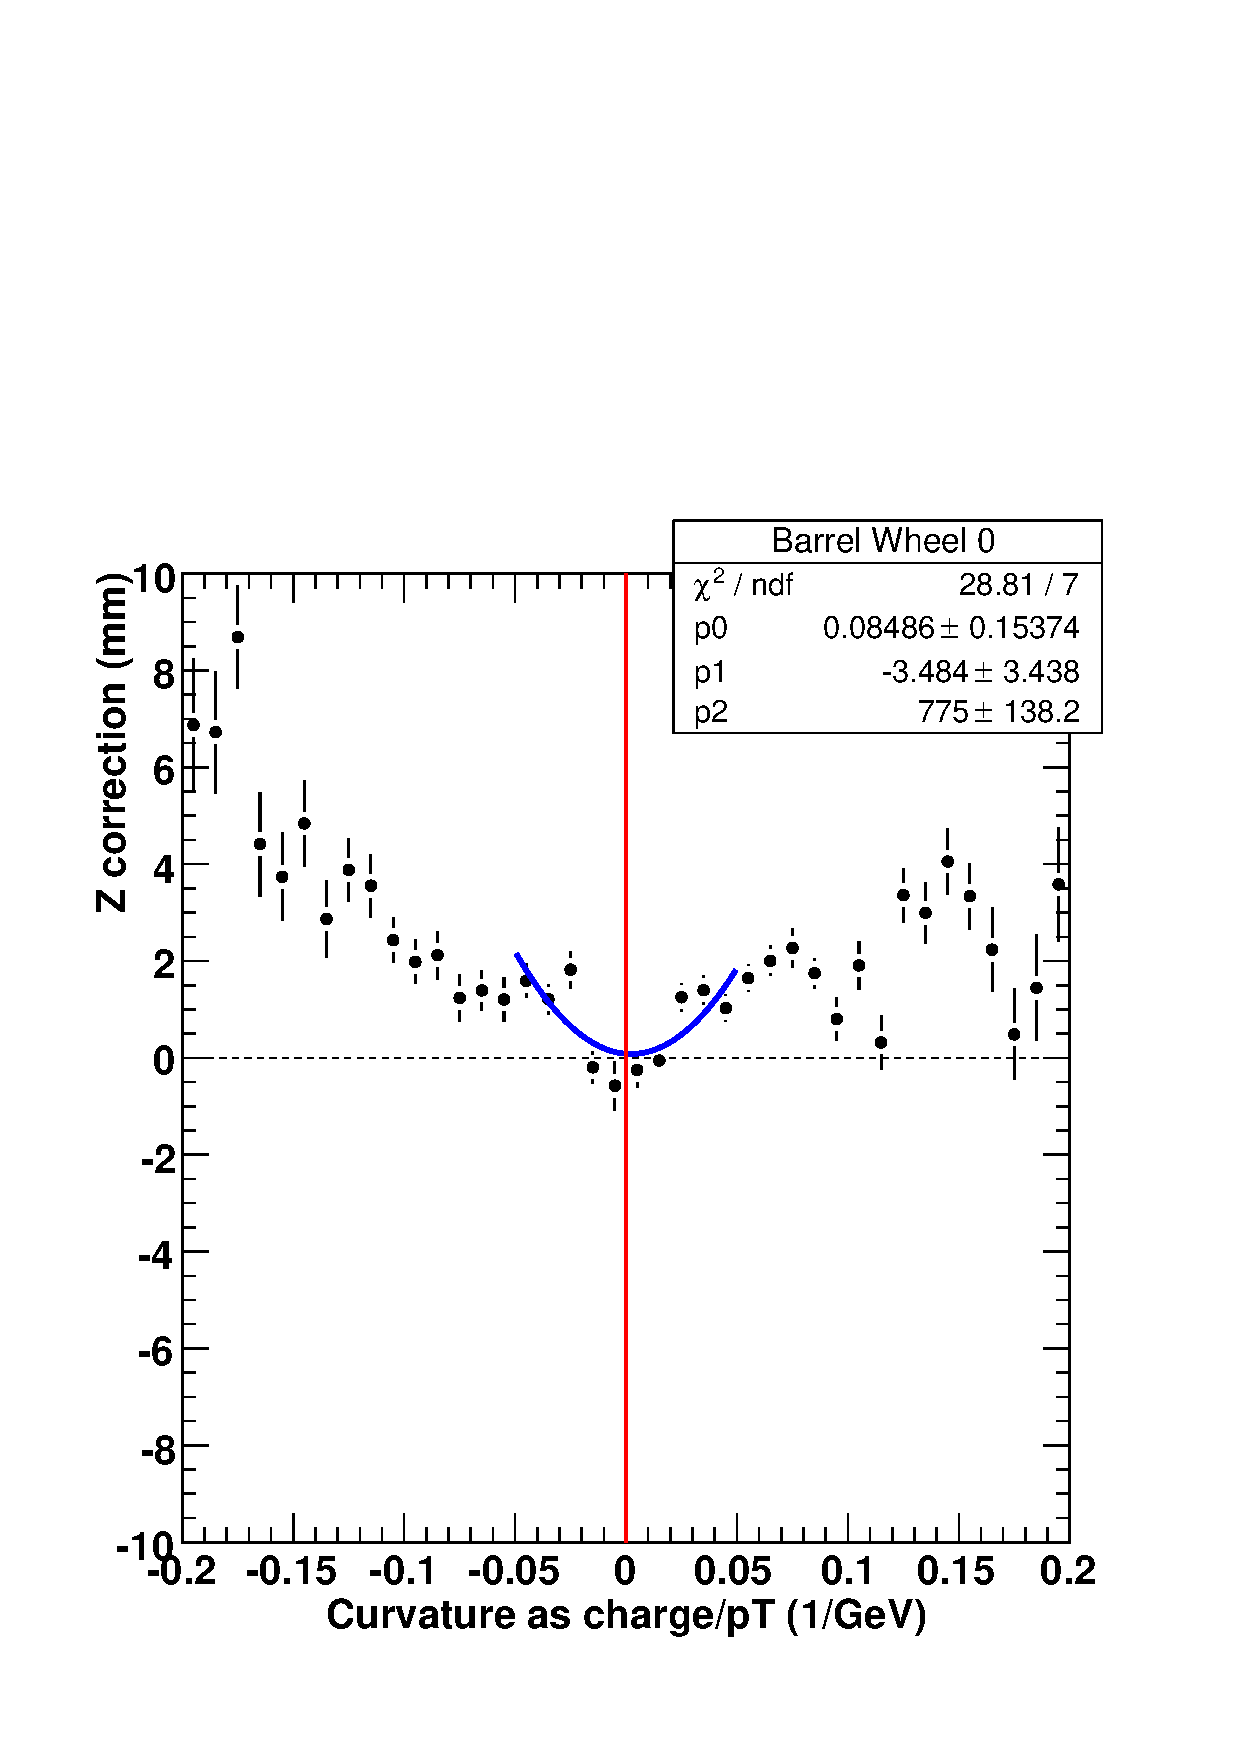
\includegraphics[width=0.8\linewidth]{ZvsCurvature_wh0_translateonly.pdf}

%% \column{0.5\linewidth}
%% 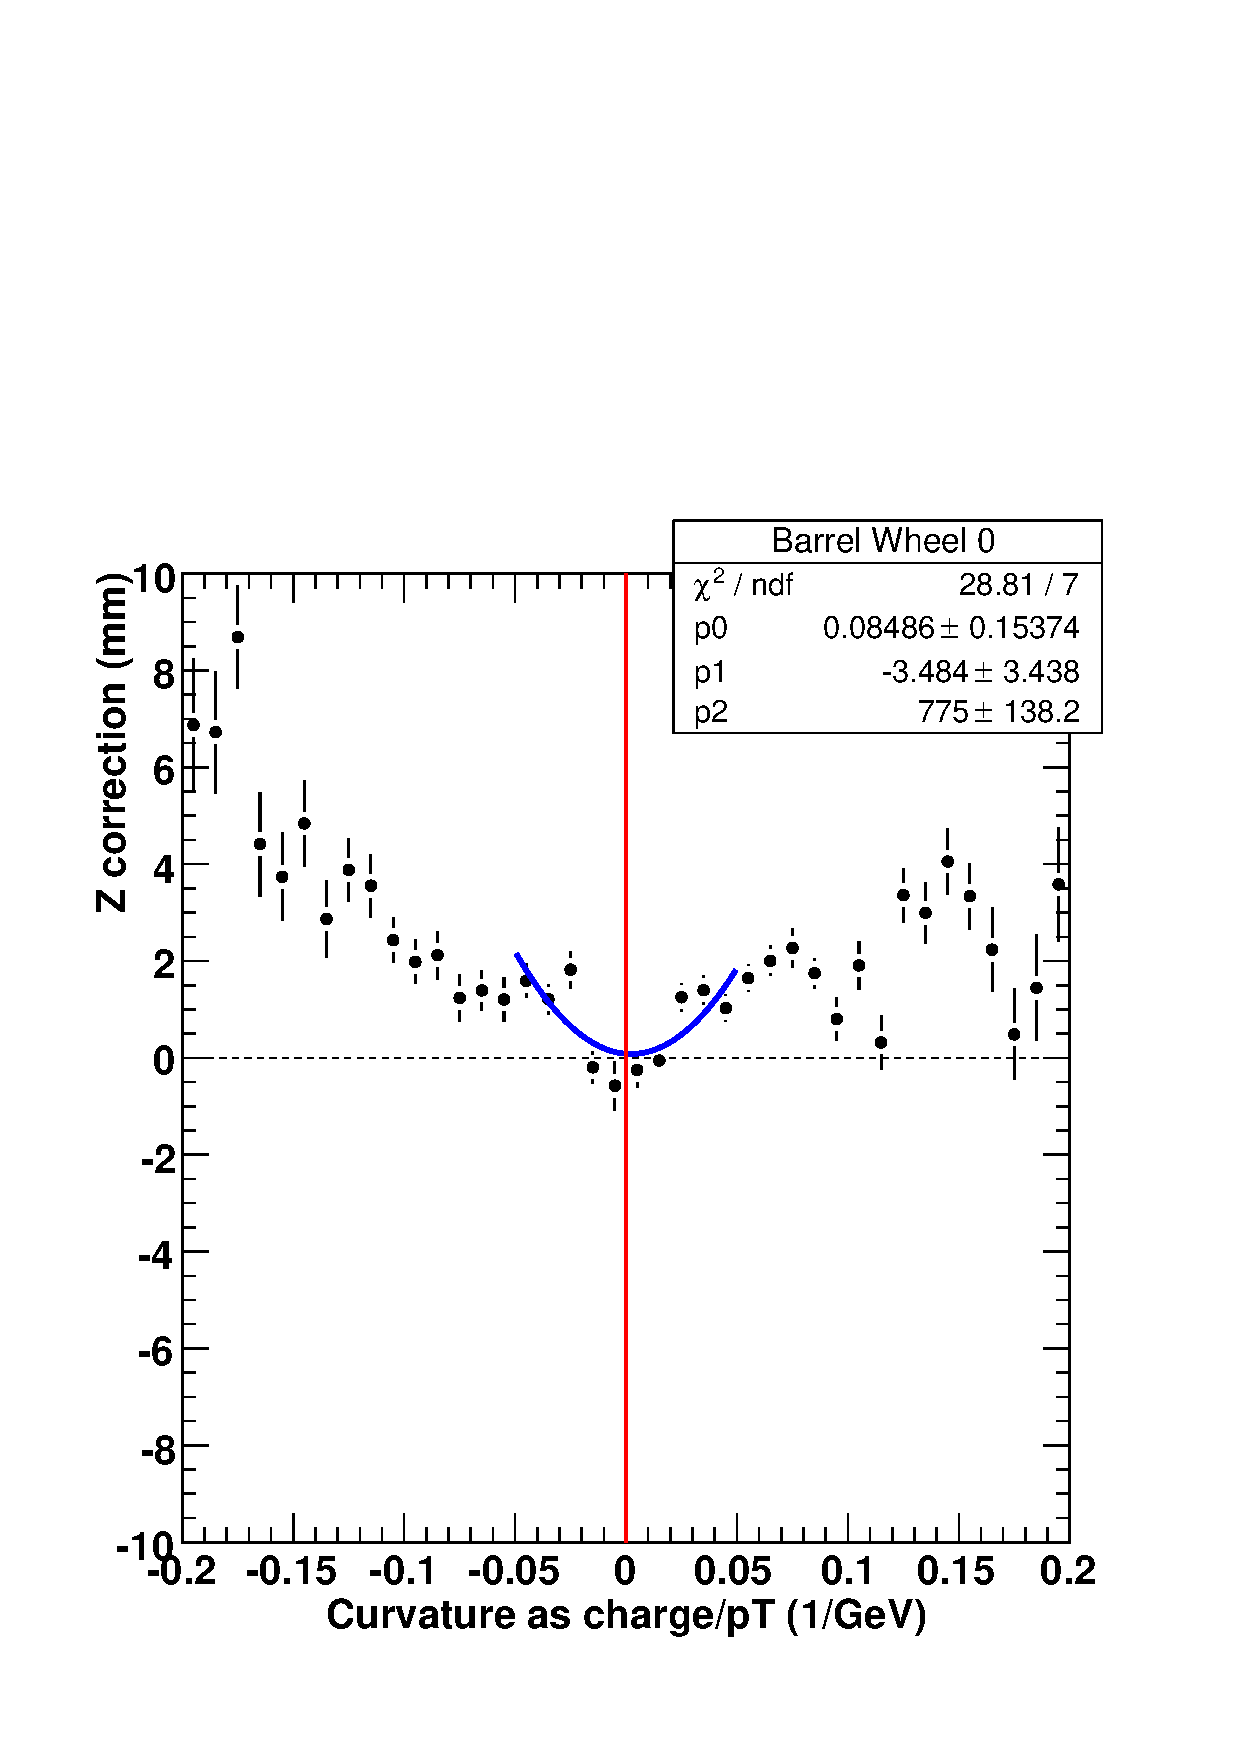
\includegraphics[width=0.8\linewidth]{ZvsCurvature_wh0_translateonly.pdf}
%% \end{columns}




%% \begin{frame}
%% \frametitle{Status of track-based procedures}
%% \begin{itemize}\setlength{\itemsep}{0.2 cm}
%% \item HIP and MillePede can produce alignments of the wheels and disks relative to the tracker with globalMuons
%% \item Constants are stable run-by-run
%% \item But they disagree with hardware constraints
%% \begin{itemize}
%% \item 2.5~mrad twist in $\phi_z$ from ME$-$2 to Wheel~0 disagrees with $\pm$0.5~mrad photogrammetry measurement
%% \item $z$ positions may or may not agree with optical measurements
%% \end{itemize}
%% \item $\chi^2$-invariant global distortions of the tracker {\it might} account for the difference
%% \item {\it If so,} track-based alignment would reverse its role and communicate physical measurements to the tracker
%% \end{itemize}
%% \end{frame}

%% \begin{frame}
%% \frametitle{Status of constants}
%% \begin{itemize}\setlength{\itemsep}{0.2 cm}
%% \item Track-based alignment moves wheels and disks as rigid bodies, so
%%   internal distortions must be supplied as input
%% \begin{itemize}\setlength{\itemsep}{0.1 cm}
%% \item Pre-CRAFT alignment of DT chambers within wheels available in CRAFT\_V3P (but updated yesterday?)
%% \item ME2,3,4 disk-curvatures from lasers were well studied but not in a
%%   CMSSW geometry record; I ported it as a public service
%% \item I received no concrete information about ME1; had to guess
%% \end{itemize}

%% \item Produced two sets of constants:
%% \begin{enumerate}\setlength{\itemsep}{0.1 cm}
%% \item Curved disks from lasers, centered whole muon system in $z$ with track-based alignment of wheel~0 \textcolor{darkblue}{(recommended)}
%% \begin{itemize}
%% \item Minimal use of track-based alignment
%% \item Global translation is not a bias but a coordinate definition
%% \end{itemize}
%% \item Curved disks from lasers, aligned wheels and disks in $z$ and $\phi_x$
%% \begin{itemize}
%% \item $\phi_x$ is difference in $z$ between top and bottom
%% \item Poor or no information on ME3 and ME4, glued them to ME2
%% \item Production was rushed!
%% \end{itemize}
%% \end{enumerate}

%% \end{itemize}
%% \end{frame}

%% \begin{frame}
%% \frametitle{Status}
%% \begin{itemize}
%% \item HIP and MillePede can produce alignments of the wheels and disks
%%   relative to the tracker with globalMuons
%% \begin{itemize}
%% \item Cosmic ray statistics are very high in wheels $-$1, 0, $+$1
%%   ($\delta z \sim 300$~$\mu$m statistical, $\sim 2$~mm systematic)
%% \item Wheel $\pm$2 and endcap disks would be better served by
%%   standAlone cosmic muons, to propagate central globalMuon alignment
%%   outward
%% \begin{itemize}
%% \item We're waiting for standAlone cosmic track refitter to be written
%%   before we can do that, so in the meantime, we produce globalMuon
%%   constants for everything
%% \end{itemize}
%% \end{itemize}

%% \item Pure track-based results were inconsistent with hardware measurements
%% \begin{itemize}
%% \item Rotations around beamline larger than what $\vec{B}$ = off photogrammetry would allow
%% \item $z$ positions along beamline might or might not be consistent with hardware measurements
%% \item Global distortions of the tracker might account for the difference
%% \end{itemize}

%% \item But you want verified constants, not procedures\ldots

%% \end{itemize}
%% %% \hspace{-0.83 cm} \textcolor{darkblue}{\Large Outline2}
%% \end{frame}

%% \section*{First section}
%% \begin{frame}
%% \begin{center}
%% \Huge \textcolor{blue}{First section}
%% \end{center}
%% \end{frame}

\end{document}
